% !TEX root = Tesi.tex
\chead{}
\chapter{State of the art}

\section{Iot Devices : RFID, NFC, Beacons and Sensors}

As per introduced in \ref{section:iot}, The Internet of Things (IoT) describes an ecosystem or network of Internet-connected objects able to collect and transfer data using embedded sensors. This ecosystem is vast but can be organized into a number of major dimensions that are discussed below : 

\begin{itemize}
  \item \textbf{Radio Frequency Identification (RFID) } is a technology predominantly applied to one-way inventory tracking and supply chain problems. Packages are affixed with passive RFID tags containing important product information that are detectable to a distance of 100 meters by stationary readers. RFID tags are comprised of a small antenna and a silicon chip capable of storing the product information to facilitate the identification.The tags are remarkably small, and can be effectively integrated with adhesive labels attached to cases and pallets, incorporated into security cards, or even implanted in pets, to name just a few examples.
  
  The primary difference with the most common electronic barcode mechanism is that barcode readers require “line-of-site”; the barcode reader must see the barcode lines to read the data and can only do that one barcode at a time while the RFID does not require it as tags can be scanned through a variety of materials. From an IoT perspective, RFID readers (that can be handheld or mounted to a specific location such as a dock door) are a powerful mechanism to read and write data across networks of RFID tags and automatic transfer vast amounts of data to any variety of data clouds or backend systems.

  \item \textbf{Near Field Communication (NFC) } comprises a set of close-range wireless communication standards offering functions similar to the most common Bluetooth and RFID technologies. Much like RFID, NFC can detect and access data from special tags but have the additional advantage of being suitable for virtually unlimited applications because information can be easily retrieved from any conventional NFC-enabled device. Similar to Bluetooth technology, NFC supports two-way secure data exchange with a simple tap or wave among devices.
  
  Currently, NFC is already incorporated into over 1 billion devices globally, including an increasing number of tablets, PCs, household appliances, electronic devices, gaming consoles and of course smartphones. For enhanced security and control, NFC operates only when devices are in close proximity (approximately 10 centimeters), thus making this technology optimal for more protected applications like financial transactions and secure login access at a particular location. 
 
  \item \textbf{Beacons} collectively refer to small wireless devices that are capable of transmitting simple radio signals embedded within a unique identification number. At any time, a nearby device such as smartphones using Bluetooth Low Energy technology detects transmitted signals resulting in the reading of the beacon's ID, calculation of the distance to the beacon and, depending on the result, may trigger an action in a beacon compatible mobile app. 
  
  Despite the simplistic mechanism, beacons represent a substantial technological advancement and have opened new opportunities to allow more precise tracking for indoor positioning and behavior compared with standard GPS technology.
  
  The simple communication associated with beacons, which importantly is not reliant on significant power consumption, unfolds a wide range of new seamless interactions with application in numerous different areas. The retail sector, for example, is currently one of the most popular fields in which beacon technology is utilized because it offers an unprecedented way to track in-store interactions between customers and product displays, ultimately resulting in more personalized offers and a better retail experience based on the acquired data. Additional applications of the beacon technology range from supporting and improving physical navigation in large spaces such as museums, airports and stadiums, to assisting impaired people in public transportation.

  \vspace{0.5cm}
  \begin{figure}[htbp]
    \centering
      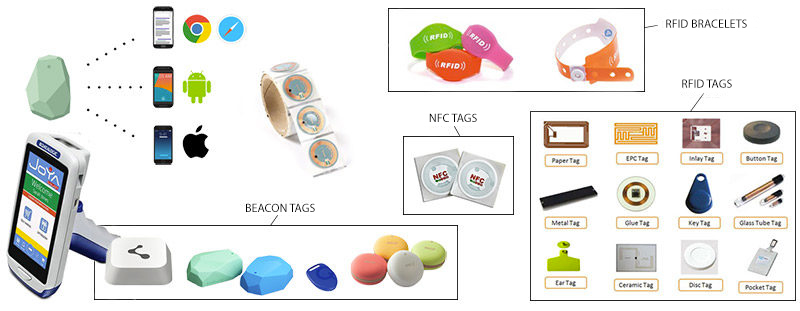
\includegraphics[height=6cm]{images/iot-devices.jpg}
    \caption{RFID, NFC and Beacon Tags}
    \label{fig:devices}
  \end{figure}
  \vspace{0.5cm}

  \item \textbf{Sensors} are physical pieces of hardware responsible for monitoring processes, taking measurements and collecting data. There are literally infinite measurements that can be gathered by sensor arrays, ranging from temperature to proximity, from pressure to water quality, and from gas detection to liquid level tracking. A wide variety of devices currently include these sensors, and based on current trends we are witnessing a move towards multi-sensors platforms capable of simultaneously incorporating different sensing elements. In the retail sector, for example, it is possible to make the store shelf "smarter" by providing visibility from the product's arrival to final sale thanks to a combination of store shelf sensors, smart displays, digital price tags and high-resolution cameras. In fact, sensor-based technology now enables the retail businesses to precisely determine product volume on store shelves and in stock rooms, leading to more efficient product ordering and restocking. A final illustration of sensor application is the next-generation of personalized self-tracking products in the form of wearables and smartwatches. Examples include combinations of accelerometers, GPS, temperature and heart rate sensors that provide a comprehensive data insight on the activity of the user.   
  

  \vspace{0.5cm}
  \begin{figure}[htbp]
    \centering
      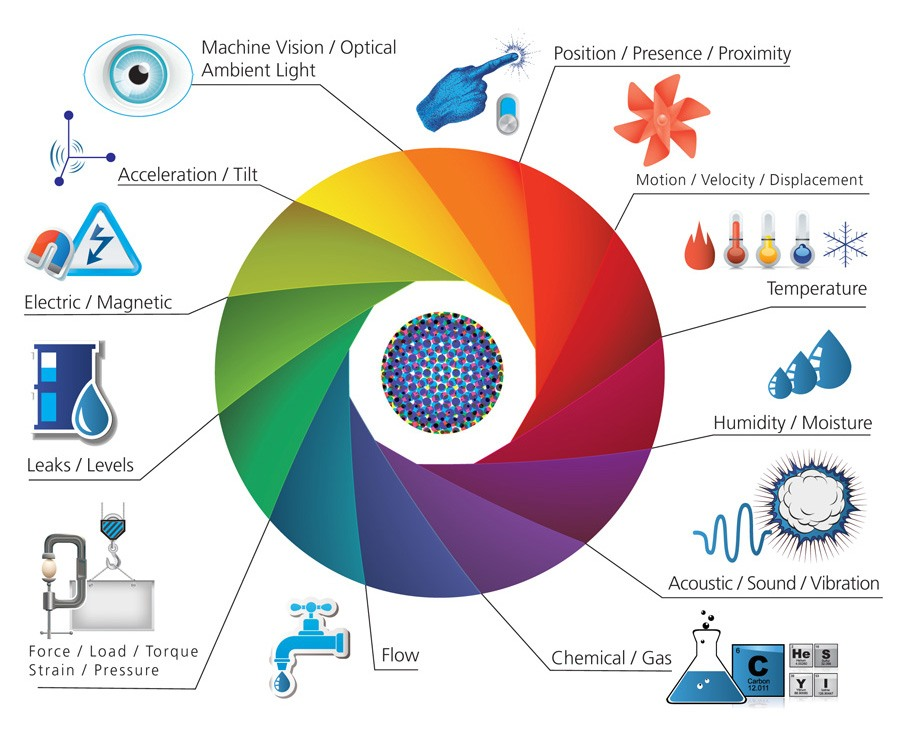
\includegraphics[height=10cm]{images/iot-sensors.jpg}
    \caption{Sensors ecosystem}
    \label{fig:sensors}
  \end{figure}
  \vspace{0.5cm}

\end{itemize} 

\section{Big Data and Predictive Analysis applications}

The concept of Big Data relates directly to the Internet of Things. Simply, IoT devices are capable of collecting terabytes of data over very short time periods, thus emphasizing the importance of being able to support the efficient processing and interpretation of data as it is collected.


It is important to note that in addition to the fact that IoT devices are capable of generating profile data at an incredibly high rate, the modern Web represents another essential data source in this paradigm (see chapter \ref{section:data-web-mining}). Social networks, for example, are capable of producing an endless stream of data describing user preferences and behaviors at any time. This vast volume of “Big Data”, available in a whole array of formats and growing constantly, provides unparalleled opportunities for addressing any number of socially-important questions.

To obtain economic value from Big Data, companies are investing in advancements in artificial intelligence and machine learning algorithms to efficiently process data, create products, and implement solutions that extend well beyond traditional systems currently used for managing and storing information. This includes novel approaches supporting high calculation inclination that are efficient at sorting data in a structured and meaningful manner to detect relationships and patterns in complex data streams. This new approach to data management differs from what companies used to do in the past when priorities were bound to an IT level governance only and they were solely accessed by a restricted set of users. Moreover, it also becomes vital for a company to identify new sources of big data when they become available on the market, and quickly incorporating them into the data management platform following a constant continuous improvement logic.

\vspace{0.5cm}
\begin{figure}[htbp]
  \centering
    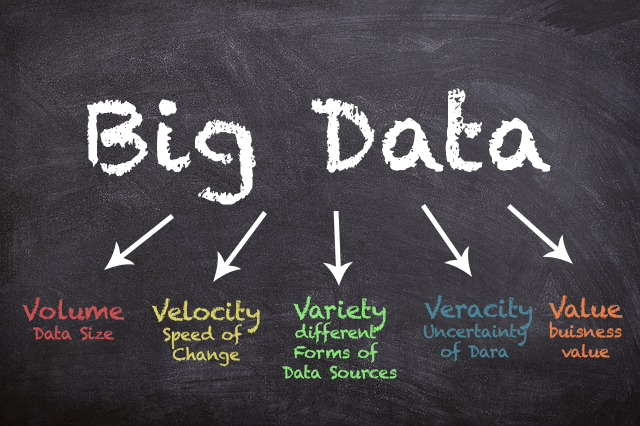
\includegraphics[height=8cm]{images/bigdata.png}
  \caption{The five fundamental Vs of big data }
  \label{fig:bigdata}
\end{figure}
\vspace{0.5cm}

Admittedly, it is challenging to forecast the added value brought by Big Data analysis to the various application disciplines in which they can be applied. However, it is clear that they certainly have improved the quality of the forecasts that contribute to more prudent decisions supported by more robust empirical evidence. 
In fact, Big Data analysis constitutes a fantastic instrument in the field of the decision-making by minimizing the risks and reducing the consequences caused by inadvertent human errors. For example, the marketing department of an organization could potentially leverage big data for increasing marketing intelligence predicting customer interests. At the same time, Big Data could be utilized to provide better forecasts of product stock replenishment and to optimize production requests.

In summary, the potential applications mentioned above represent the core of the predictive analysis notion: the practice of extracting information from Big Data with the goal of determining patterns and predicting future outcomes and possible trends. 

It is also important to remark that this kind of analysis does not offer a precise assessment of what will occur in the future but rather they forecast the likelihood of particular outcomes with an acceptable level of reliability. This often includes what-if scenarios and risk assessments.

Focusing on the Marketing intelligence example mentioned above, the benefits of using Predictive Analysis are important to fully understand. Recently, digital companies are increasingly embracing this idea because it offers a better and more constructive experience to the customers on every possible point of contact between the business itself and the clients. This can increase customer loyalty and, by extension, economic returns.

\vspace{0.5cm}
\begin{figure}[htbp]
  \centering
    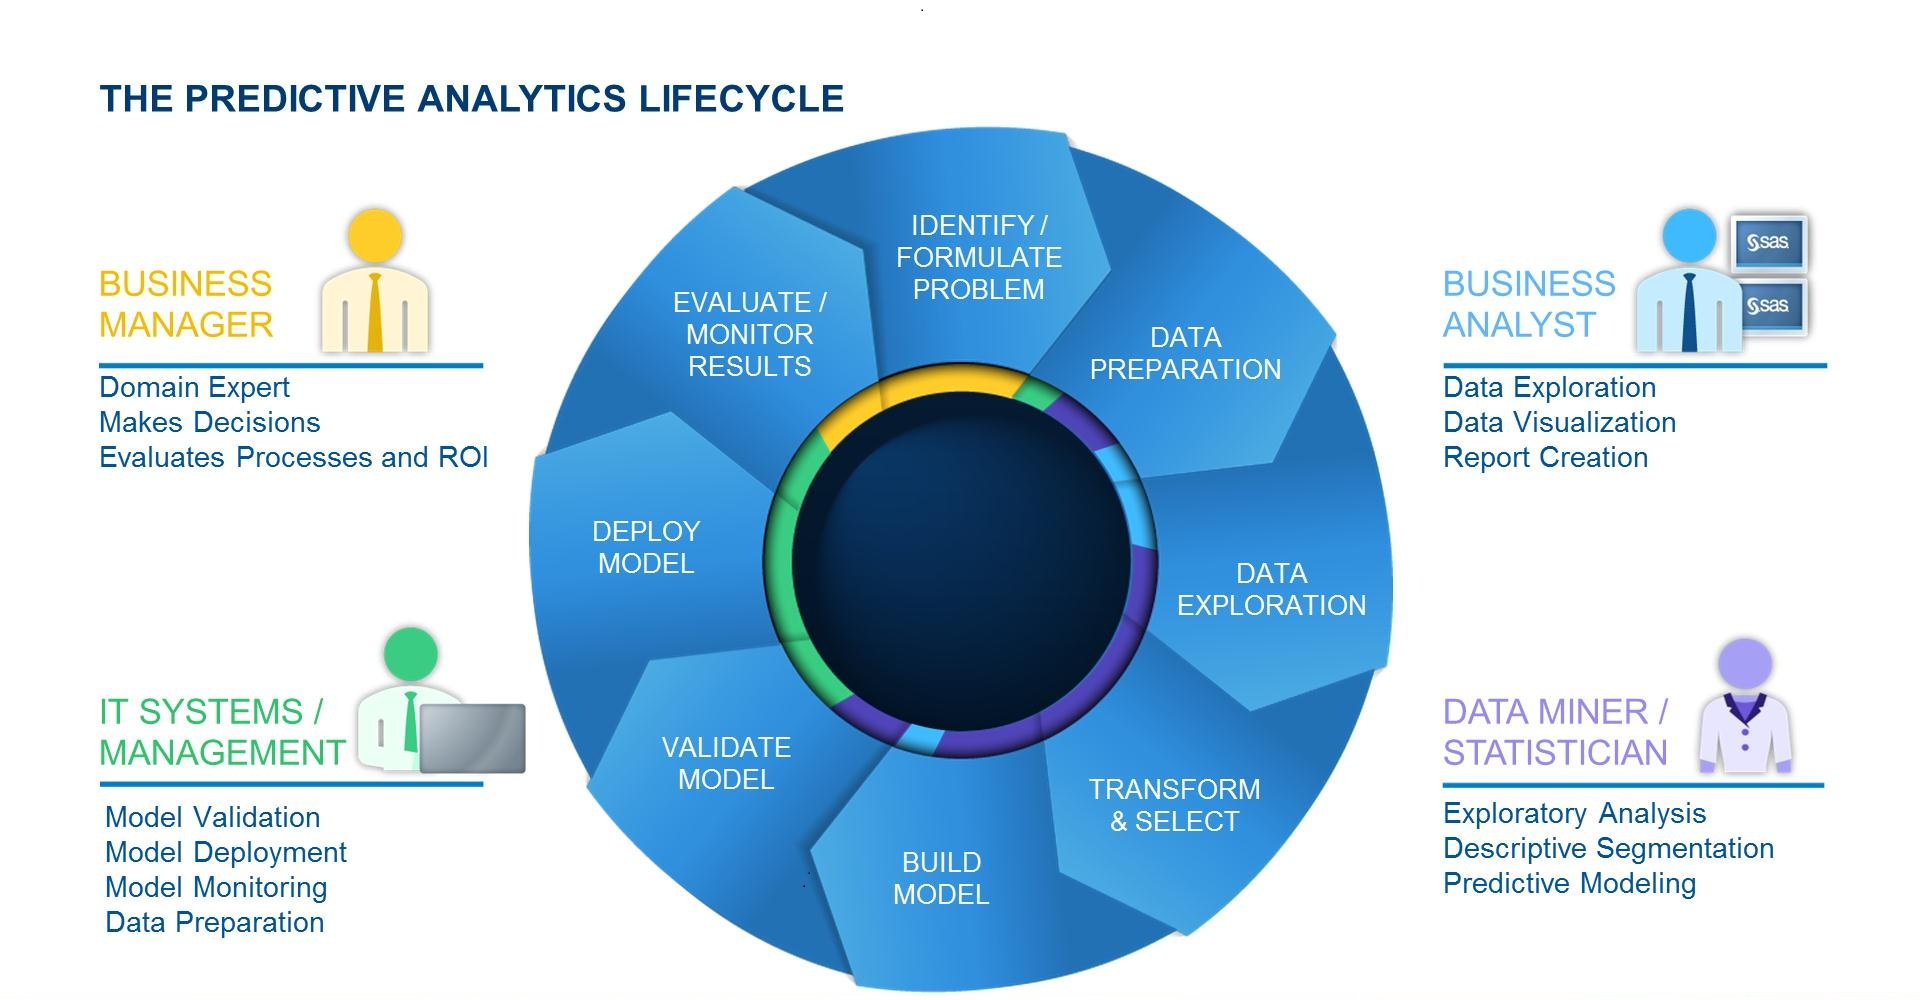
\includegraphics[height=8cm]{images/pa-lifecycle.jpg}
  \caption{The predictive analysis lifecycle }
  \label{fig:bigdata}
\end{figure}
\vspace{0.5cm}


In more detail, this outcome can be achieved using sophisticated algorithms and mathematical models on top of the big datasets of customers activity accessible from Big Data sources; eventually, this data gets sanitized, structured and filtered and finally grouped in a meaningful way. 

The behaviors and patterns of interaction detected by this analysis process can indicate, for example, a more appealing product offer with a major chance of conversion for a particular customer profile segment.

Different typologies and techniques are used to perform enhanced analysis for behavioral prediction. Here, I discuss a few of the major approaches.

\begin{itemize}
    \item \textbf{Clustering or Unsupervised learning}:  This methodology seeks to group similar individuals and identifies with high precision based upon the enterprise's customer base. These algorithms can process hundreds of attributes with the goal of identifying those characteristics that best discriminate individuals according to their behavior. The underlying notion is that, statistically, distinct groups of individuals behave in similar ways. 
    
    Group clusters obtained with this process are similar to groups determined through a priori classification; the only fundamental difference between the two methodologies is that clustering or unsupervised learning allows individuals to be categorized into different groups based solely on data and not pre-conceived attribute differences. 
    
    Clusters can be of different types depending mostly on the criteria by which customers are grouped. Product-based clusters, for example, collate all customers who tend to buy products or combinations of several products in the same category. By contrast, brand-based clusters focus on grouping customers who prefer certain brands instead of others, and behavior-based clusters combine consumers with similar buying behaviors, helping the marketing manager to identify the most appropriate way to address each of them.

    \item \textbf{Propensity models or Supervised learning}: This family of techniques is based on probabilistic models using advanced machine learning techniques such as neural networks, logistic regression, random forest, and genetic algorithms. The main purpose of these procedures is to predict future customer behavior based on past examples. Over time, these algorithms become more efficient, improving predictions when more data is collected.

    \item \textbf{Reinforcement learning and Collaborative filtering}: This increasingly popular technique has been demonstrated in a number of major applications, one of the most famous being the ability of companies to recommend products to purchase. The recommendations are targeted and tailor-made for the client and they are defined by considering the entire relationship between customer and brand. For this reason, they can upsell for higher value products, cross-sell to same category items or dynamically link to other products based on the modeled associations.
  \end{itemize} 

%\addcontentsline{toc}{chapter}{}
